\subsection{Marzo}
\subsubsection{Informe 13/3}
Prueba del sensor HW-666 (medidor de corriente)\\

          	Para esto, se utilizó un alargue, al cual le sacamos el conector hembra y 30 centímetros del aislante exterior, quedando libres los 3 cables que posee.\\
          	El cable marrón (línea) se pasó a través del sensor, y luego se volvió a armar el conector hembra. De esta manera, poseemos un conector hembra con conexión a 220, y la corriente que fluya a través de este podrá ser medida por el sensor.\\
           
          	Probamos la medición de corriente con una pistola de calor, una estufa eléctrica y un soldador, y medimos la señal de salida con un osciloscopio digital.\\
           
          	En las mediciones que realizamos, pudimos aproximar correctamente la corriente con una precisión aproximada del 10\%, comparando la corriente teórica en base al consumo teórico con la corriente calculada y el consumo calculado. Próximamente se buscará conseguir una pinza amperimétrica para ver realmente el error del sensor.\\
           
          	A través de diversas pruebas, y también basándonos en la información brindada por el vendedor, concluimos que la corriente máxima que puede medir el sensor sin distorsionar la señal de salida es de alrededor de 5 Amper. Si queremos aumentar la corriente máxima medida a 10 Amper, hay que cambiar la resistencia SMD del sensor a una de 100$\Omega$ (actualmente posee una de $200\Omega$). Adjunto fotos de la prueba y la información brindada por el vendedor.\\
 
Características:
\begin{itemize}

\item Transformador de corriente de 5A a 5mA
\item Resistencia de carga incluida de 200 Ohm
\item Relación de vueltas: 1000: 1
\item El rango lineal: 0 ~ 10A (Sobre una resistencia de carga de 100 Ohm)
\item Linealidad: 0.2% (Sobre una resistencia de carga de 100 Ohm)
\item Error de ángulo de fase= Menor a 20° (Sobre una resistencia de carga de 100 Ohm)
\item Tensión de aislamiento: 3000 V
\item Sellado material: Resina epoxi
\item Temperatura de funcionamiento: -40°C a 70°C
\item Montaje: M2 12mm
\item Pines de Salida: 2.54mm

\end{itemize}


\begin{figure}[H]

\begin{subfigure}{0.5\textwidth}
\includegraphics[width=0.9\linewidth]{informes/IMG_7659.jpg} 
\caption{Circuito probado.}
\end{subfigure}
\begin{subfigure}{0.5\textwidth}
\includegraphics[width=0.9\linewidth]{informes/IMG_7660.jpg}
\caption{Señal de salida del sensor.}
\end{subfigure}
\end{figure}

\begin{figure}[H]
    \centering
    \includegraphics[width=0.75\linewidth]{informes/Screenshot_10.jpg}
    \caption{Conexión del sensor}
\end{figure}

Prueba del ADC externo ADS1115:\\

En esta prueba, utilizamos un ADC1115 (datasheet) como ADC externo de 16 bits conectado por i2c (que puede funcionar con 3.3V y 5V) al micro ESP32. Para eso, buscamos una librería preparada para micropython que nos facilite el uso del ADC externo, y encontramos esta en GitHub, que fue la que terminamos instalando y usando. Lo probamos midiendo un voltaje de continua a la entrada A0 del ADC externo, entonces comparamos lo que nos otorga el micro luego de recibir y procesar la lectura del ADC externo con la medición del tester. Como se puede ver en una de las imágenes adjuntas a esta explicación, las mediciones de voltaje entre el tester y el ADC externo son prácticamente iguales. \\

Sin embargo nos encontramos con un par de inconvenientes:
Si queremos que el ADC pueda medir valores de hasta 5V en sus entradas, tenemos que alimentarlo con 5V, y eso implica que intentará comunicarse en i2c con 5V al micro (la ESP32 acepta en sus pines una entrada máxima de 3.3V). La solución sería usar un divisor resistivo de tensión para los cables de SDA y SCL que van al micro.
Como requerimos medir alterna, tendremos que medir voltajes diferenciales con el ADC, lo que implica usar 2 entradas por señal.\\

El ADC nos entregaba valores no concordantes. Para 3.3V, que debería ser el máximo que puede medir porque con eso lo alimentamos (por tanto correspondería al bit más alto de la medición) nos entregaba un piso equivalente a menos de la mitad (En vez de valor 65000 entregaba valor 26000). En su momento se resolvió tomando ese valor que entregaba (26000) como bit máximo en lugar de los 65000 (es un ADC de 16 bits, por tanto $2^16$) y se solventó el problema, pero perdimos resolución (aunque a estas escalas no es muy relevante). La posible respuesta es que el ADC tiene Vrefs fijas, no es la de alimentación, y según el caso puede dividir las tensiones en fracciones a la hora de mostrar resultados (o a eso apunta el datasheet). Por tanto se corregiría configurando el ADC a cierta Vref y usar esa tensión en lugar de 3.3V en el cálculo que hace el micro para estimar el voltaje (por ejemplo no tiene 5V, tiene 4.096V o 6.144V).\\

Bajo esta línea, nuestro próximo objetivo es lograr un código en la ESP que, al conectarle el sensor de corriente (este midiendo la corriente en un cable de 220V 50Hz), pueda tomar varios valores de corriente alterna por ciclo (varios por cada 20mS), los enliste, y separe el más alto, así tendríamos una medición de la Ipico que pasa por el cable. \\

\begin{listing}[H]
\begin{minted}{python}
import ads1115
from machine import I2C, Pin
import time

i2c = I2C(1, scl=Pin(22), sda=Pin(21), freq=400000) #i2c setup

adc = ads1115.ADS1115(i2c, 72, 0) #activo mediciones con el adc externo
 
voltaje = adc.raw_to_v(adc.read(4,0)) #calculo de voltaje, samples default
print(voltaje)
\end{minted}
\caption{Lectura de voltaje con ADC externo}
\label{lectura ads 1115}
\end{listing}

\begin{figure}[H]
    \centering
    \includegraphics[width=0.65\linewidth]{informes/IMG_7678.jpg}
    \caption{}
\end{figure}

\begin{figure}[H]
    \centering
    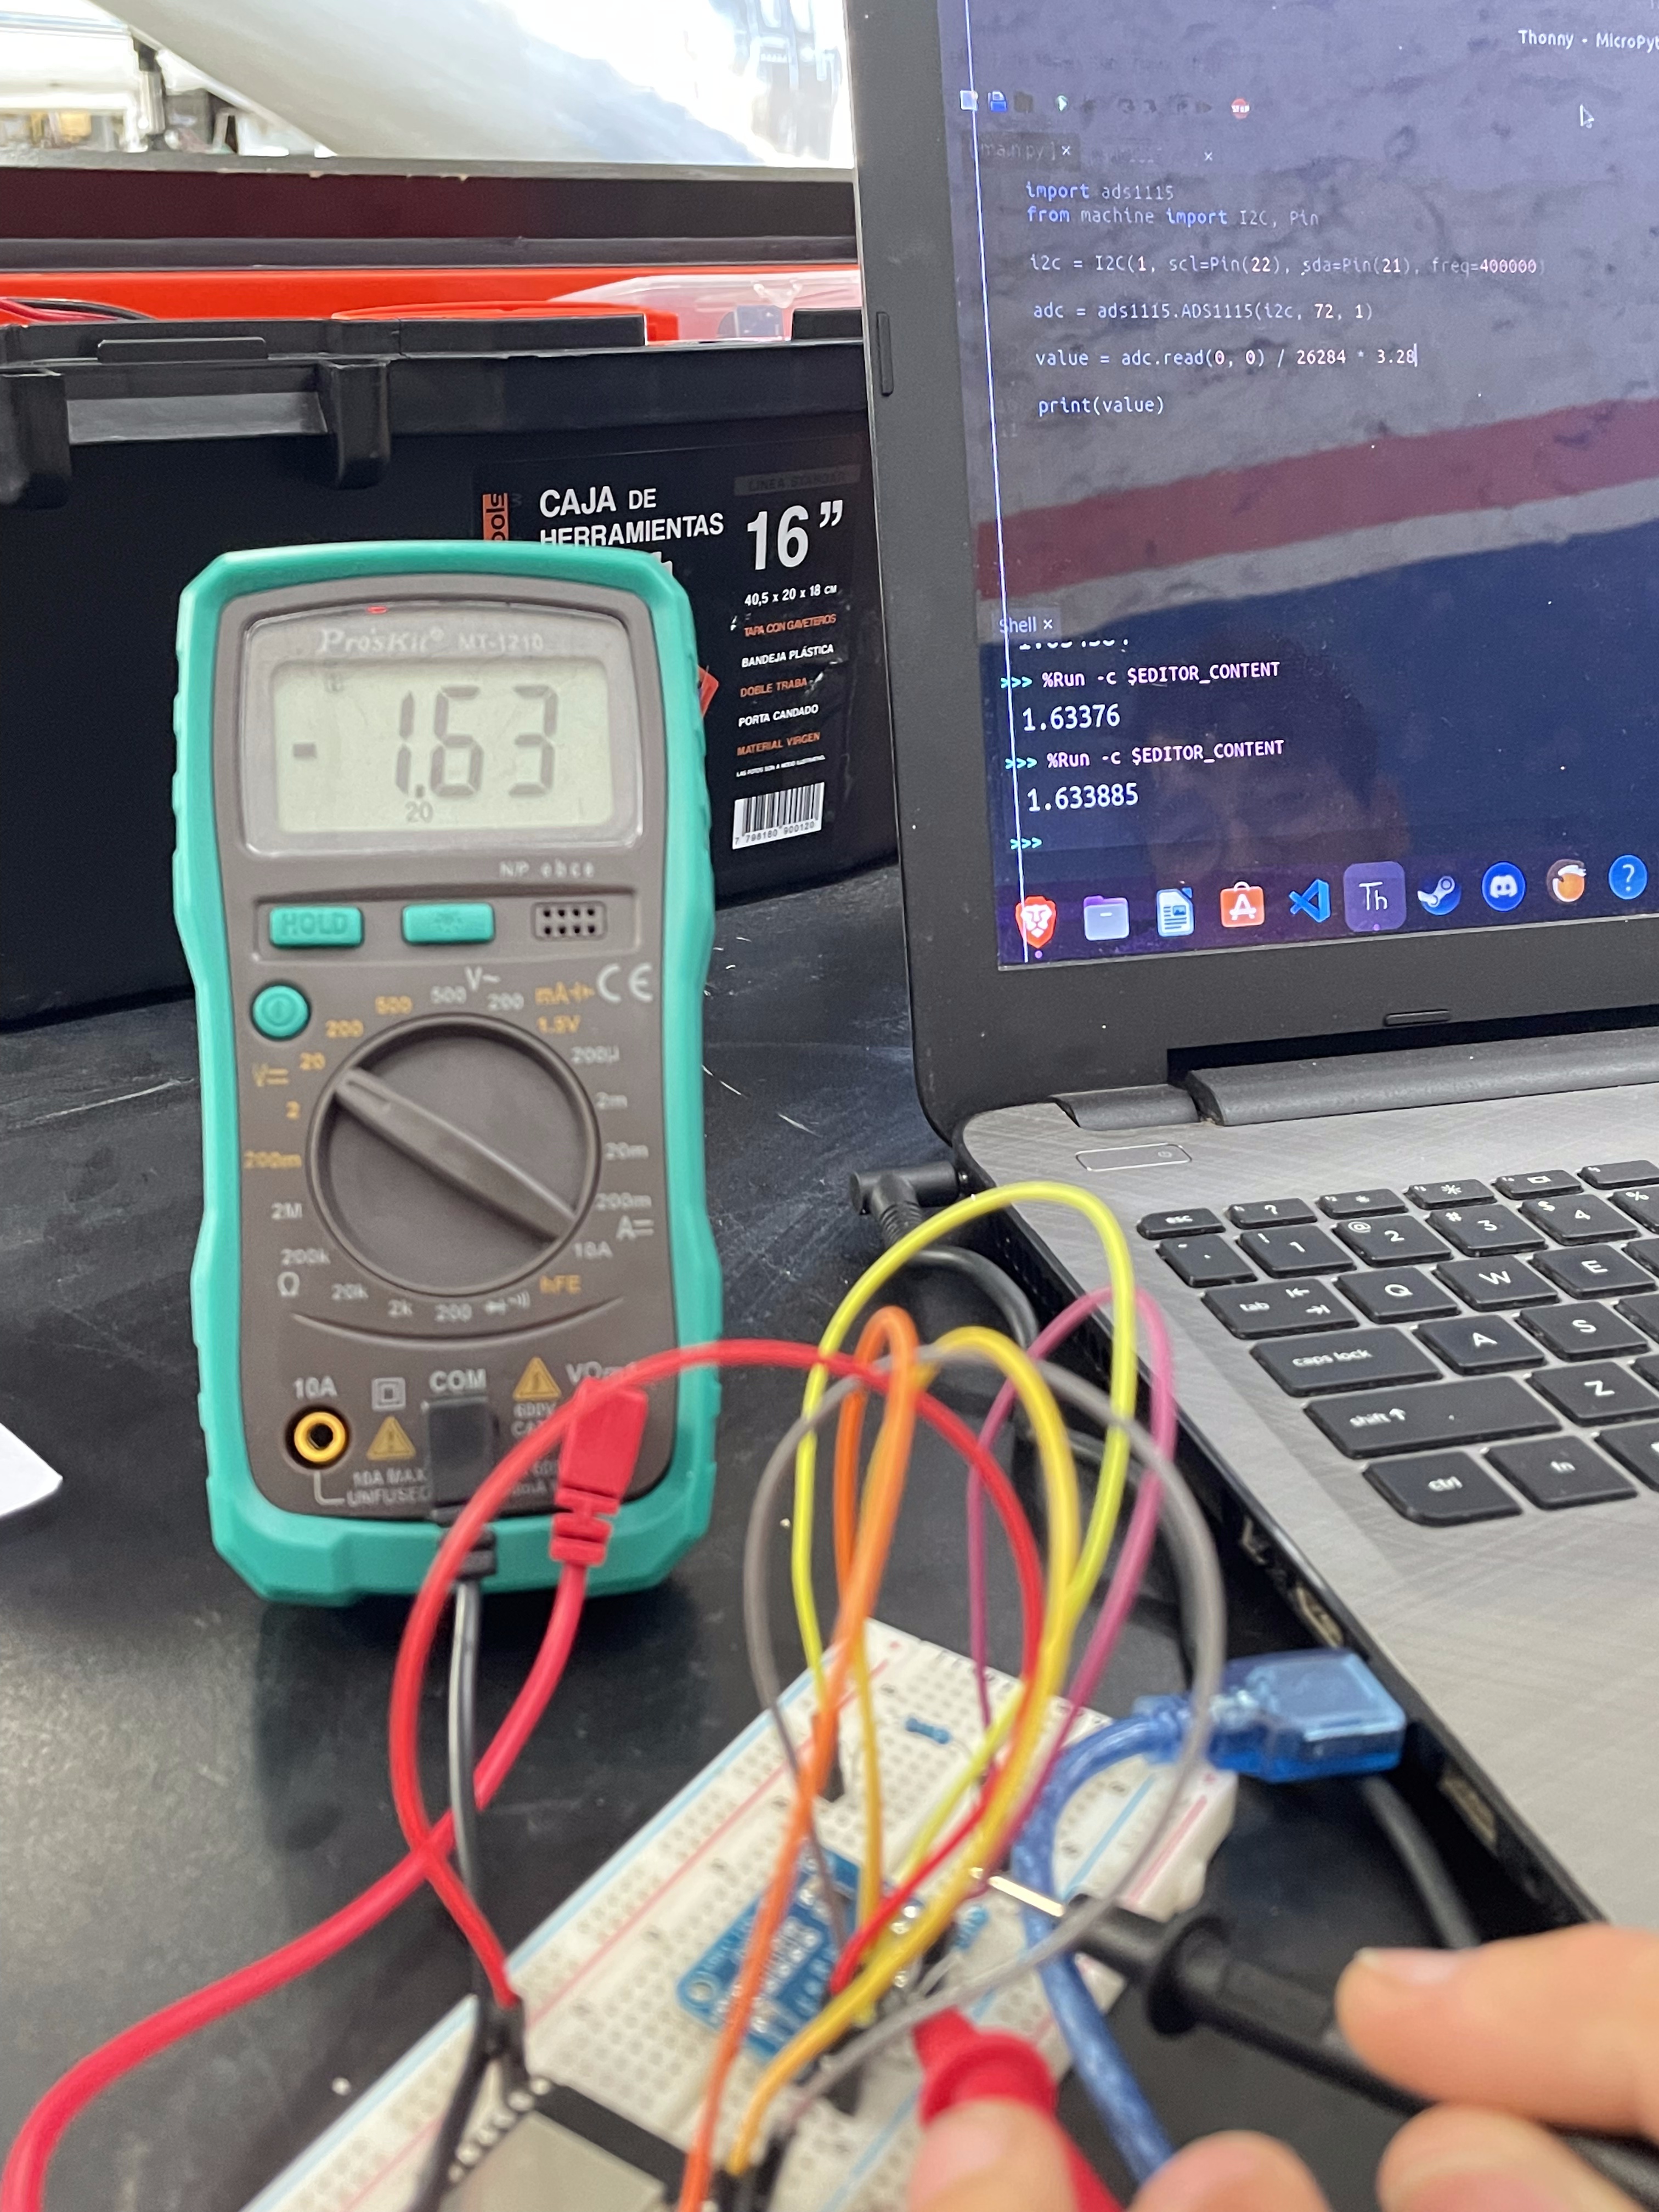
\includegraphics[width=0.75\linewidth]{informes/IMG_7684.jpg}
    \caption{Medición del ADC}
\end{figure}


\subsubsection{Informe 20/3}

Medición de corriente:

En este día, nos encargamos de utilizar el ADS1115, el sensor de corriente y la ESP32 para medir la corriente que pasa por un cable que alimenta una estufa. La idea era compararlo con una pinza amperométrica para ver si las mediciones de corriente pico eran adecuadas. Nos encontramos con varios problemas:
\begin{itemize}
\item No conocemos la escala del sensor (no hay documentación disponible), pudimos aproximarlo a partir de cálculos con valores conocidos, pero nos generó un error en la medición cuando había corrientes altas, de 3 amperes para arriba (posiblemente no tenga respuesta lineal).
\item La pinza amperométrica nos resultó volátil, podía cambiar los valores en 0.4 amperes de repente, lo cual nos dio desconfianza a la hora de saber realmente cuánta corriente pasaba por el cable, y si era correcto el sensor conectado a la ESP o la pinza.\\
\end{itemize}

Una vez logradas unas mediciones que considerábamos más o menos válidas, ya que en corrientes bajas no había diferencia entre el sensor y la pinza, fuimos a comprobar qué tan veloz era la respuesta del sistema sensor-ADC-ESP32 (La señal que queremos medir son voltajes de línea que tienen 50Hz de frecuencia, por tanto el sistema tiene que ser mucho más rapido que 20mS, un ciclo de onda de 50Hz, para que pueda sacar varias muestras de la señal, y podamos tener una muestra de la corriente pico “fidedigna”). Para esto ideamos que el micro haga una lista de los valores que mide, y luego con un código de Python aparte, nos grafique eso respecto del tiempo que calculamos que iba a tomar cada muestra (estimamos 1mseg), a ver si quedaba aproximadamente senoidal. Para esto usamos las librerías numpy y Matplotlib (documentación usada). Aquí se nos cruzaron varios problemas:
\begin{itemize}
\item Hicimos los cálculos para saber a qué tiempo se refiere cada muestra. Resultó algo medio ilógico, ya que nosotros habíamos calculado para que grafique una onda sola, y nos graficó un poco más de dos. Cabe mencionar que el eje “y” corresponde al voltaje que entrega el sensor, no corresponde a un valor de corriente aún, pero sirve igual porque ambos tienen la misma respuesta, solo cambiaría la escala de valores.\\
\end{itemize}

\begin{figure}[H]
    \centering
    \includegraphics[width=0.75\linewidth]{informes/Screenshot_1.jpg}
    \caption{Gráfica de corriente.}
\end{figure}


Esto se resolvió al entender que seguramente el cálculo no consideró el tiempo que toma la transmisión por i2c y el procesamiento del micro con micropython. Luego de hacer una consideración un poco más aproximada, quedó así:\\

\begin{figure}[H]
    \centering
    \includegraphics[width=0.75\linewidth]{informes/Screenshot_2.jpg}
    \caption{Gráfica de corriente con base de tiempo corregida.}
\end{figure}

Obsérvese que es la misma gráfica, solo que ahora las unidades de tiempo tienen más sentido.\\

De quererse una medición más exacta, habría que medir el tiempo que toma cada medición y asociarlo al valor de voltaje que nos dice el ADC, de esta forma se tendría una coordenada por medición y sería super exacto, sin embargo no es de interés por el momento, ya que solo necesitamos los picos de corriente para a futuro poder sacar la potencia.\\

Una vez visto esto, proseguimos a sacar lo que nos interesaba, el valor de corriente pico. Para eso en el código ideamos que se tomen varias muestras como las anteriores, de cada una se saque el valor máximo, y después comparen cada toma máxima y se tome la máxima entre ellas. Así se consigue el valor pico más exacto posible.\\

Códigos:\\

\begin{listing}[H]
\begin{minted}{python}
import ads1115
from machine import I2C, Pin
import time
import math

list = []
maximos_voltajes = []
voltaje = 0
maximo = 0
res = 0
i2c = I2C(1, scl=Pin(22), sda=Pin(21), freq=400000) #i2c setup

adc = ads1115.ADS1115(i2c, 72, 0) #activo mediciones con el adc externo

for _ in range(10): #10 muestras de señales
    while len(list) < 20: #20 muestras de voltaje
        voltaje = adc.raw_to_v(adc.read(7,0,1)) #paso a voltaje
        list.append(voltaje) #añado a la lista de voltajes de esta muestra
    maximo = max(list) #saco el maximo de esta muestra
    maximos_voltajes.append(maximo) #lo apendo a la lista de máximos
    list = [] #vacio la lista de muestras de voltaje

res = max(maximos_voltajes) / math.sqrt(2) / 0.31 #calculo corriente eficaz
print(res)
\end{minted}
\caption{Lectura ADC ESP 32}
\label{ads1115 lectura 2}
\end{listing}

\begin{listing}[H]
\begin{minted}{python}
    import numpy as np
from matplotlib import pyplot as plt

list_x = []
list_y = [-0.04875149, -0.09112779, -0.07106466, -0.002812586, 
0.07012713, 0.09225282, 0.05006403, -0.02662581, -0.08569011, 
-0.08400256, -0.02568829, 0.05268911, 0.09169029, 0.06843959, 
-0.0007500229, -0.07293972, -0.0918778, -0.04781396, 0.02981341, 
0.08700266]

num = 0
for i in range(20): #genero valores de tiempo
   list_x.append(num)
   num += 1/860 + 0.001

x = np.array(list_x) #eje x
y = np.array(list_y) #eje y

#propiedades de la grafica
plt.title('Medicion de corriente')
plt.xlabel('Tiempo (segs)')
plt.ylabel('Corriente pico')
plt.plot(list_x, list_y) #plot
plt.savefig("grafico.png")
\end{minted}
\caption{Programa en python para graficar}
\label{grafica en python}
\end{listing}

Además, armamos un segundo alargue con el otro sensor para posteriormente medir los dos sensores en paralelo, y un portalámparas para medir corrientes de menor proporción.\\

\subsubsection{Informe 27/3}

Puesta a punto del espacio de trabajo:\\

Reparamos la mesa de trabajo, el zócalo que estaba en el borde posterior completamente suelto que incomodaba y parecía hasta cierto punto peligroso. Lo retiramos junto con los tornillos que lo sostenían, y cambiamos la disposición del zócalo, ahora siendo sostenido contra la base de la mesa (en lugar de sobre esta), con tornillos nuevos y totalmente encolado.\\

Medición de consumo:\\

En el día de la fecha convertimos las mediciones de corriente en mediciones de consumo (potencia eléctrica), y lo testeamos con una estufa, un soldador y una lámpara de 76W.\\

Esta vez, conseguimos un amperímetro más confiable para usar de referencia, el cuál usamos para sacar una constante que, al multiplicarse por el voltaje pico que entrega el sensor, directamente nos dé la potencia, gracias a sacar una serie de “puntos de referencia” (sacamos la potencia real de la lamparita y la estufa con el multímetro, y la dividimos con el voltaje que entregaba el sensor al medir el cable que alimentaba la lamparita o estufa, el resultado de la operación sería equivalente al último paso de una regla de 3. Por tanto habría que multiplicarlo por el valor medido del sensor, para que como resultado dé la potencia de lo que sea que se esté midiendo en ese momento).\\

En este punto nos encontramos con un problema importante: como ya se había anticipado, el sensor no tiene respuesta lineal. Aún así, es bastante próximo y dejamos la solución para después. Entonces procedimos a usar esta constante aproximada para que el código muestre en tiempo real (una medición por segundo) la potencia medida de lo que se carga al cable. El código de la ESP es el siguiente:\\

\begin{listing}[H]
\begin{minted}{python}
import ads1115
from machine import I2C, Pin
import time
import math




list = []
i2c = I2C(1, scl=Pin(22), sda=Pin(21), freq=400000) #i2c setup


adc = ads1115.ADS1115(i2c, 72, 0) #activo mediciones con el adc externo


while 1:
   voltaje = adc.raw_to_v(adc.read(7,0,1)) #medición voltaje
   list.append(voltaje) #lista de voltajes
  
   if len(list) == 333: #si se tomaron 333 muestras (aprox 1 seg)
       v_max = max(list) #busco el valor más alto
       list = []
       res = v_max * 820 #cte para convertir a potencia
       print(res)
\end{minted}
\caption{Conversión a potencia a partir de los valores del sensor}
\label{conversion directa a potencia}
\end{listing}

Para resolver el problema de la escala no lineal del sensor utilizamos un método matemático que permite generar una función que tenga una respuesta muy similar a los puntos de coordenadas que se le proporcionen. En este caso lo hicimos con Python y le pedimos al código que la función aproximada sea de grado 3 (mientras mayor grado, más precisa). La función de Python se llama Polyfit y es de la librería numpy, adjuntamos documentación de numpy usada en esta ocasión, omitiendo la de polyfit ya adjuntada:\\
\begin{itemize}
\item Aplicación del método matemático con Python y gráfico con matplotlib
\item Plot de funciones con matplotlib
\item Potencias con el módulo math de Python
\end{itemize}

\begin{figure}[H]
    \centering
    \includegraphics[width=0.75\linewidth]{informes/Screenshot_4.jpg}
    \caption{Función generada a partir de los puntos obtenidos.}
\end{figure}
\begin{listing}[H]
\begin{minted}{python}
import numpy as np
from matplotlib import pyplot as plt
import math


list_x = [0, 0.09, 0.77, 1.14]  #voltajes en el sensor
list_y = [0, 76, 716, 1141] # potencias asociadas a los voltajes en el sensor
coeficientes = np.polyfit(list_x, list_y, 3) #coeficientes de la funcion


x = np.array([0, 0.09, 0.77, 1.14]) #objeto array de numpy con el eje x
y = coeficientes[0] * pow(x,3) + coeficientes[1] * pow(x,2) + coeficientes[2] 
                                * x + coeficientes[3] #la función equivalente


plt.plot(x, y)
plt.show()
plt.savefig("respuesta del sensor.png")
\end{minted}
\caption{Generación de la función aproximada}
\label{generacion de funcion aprox}
\end{listing}

Esto se aplicará en un futuro al código de la ESP, incluyendo directamente la función en el código.


\subsubsection{Informe 31/3}

Diseño de PCB

Se diseñó la primera plaqueta del proyecto, siendo esta el módulo para medir corriente. Ingresa una alimentación de 3,3V y sale una señal de i2c para el microcontrolador. La plaqueta posee los dos sensores de corriente, los cuales hay que atravesarlos el cable de línea de la fase a medir, el adc externo, que mide los sensores, y un led, que indica si la placa está siendo alimentada. Se agregó una capa de aislamiento, la cual está conectada al negativo de la alimentación, funcionando como masa y evitando todo el ruido posible. \\

\begin{figure}[H]
    \centering
    \includegraphics[width=0.75\linewidth]{informes/Screenshot_16.jpg}
    \caption{Esquemático}
\end{figure}

\begin{figure}[H]
    \centering
    \includegraphics[width=0.75\linewidth]{informes/Screenshot_17.jpg}
    \caption{PCB}
\end{figure}

Como el sensor de corriente no está en las librerías de Kicad, se reemplazaron por conectores en el esquemático, y por pines de 2 patas. Se marcaron los agujeros en las esquinas de 4 mm para taladrar y poder colocar la plaqueta, y se etiquetó con nombre del proyecto y de plaqueta.\\

\subsection{Abril}

\subsubsection{Informe 5/4}

Desarrollo de página web:\\

El proyecto, como requiere de una aplicación, también necesita de una página web. La aplicación será diseñada como una web app, por lo que desde la página, además de poder acceder a contenido básico como información, contacto, y otros, también se la utilizará para inicio de sesión y gestión de datos asociados a cada usuario de SolarLink.\\

Lo trabajado al día de la fecha se encontrará en el siguiente link (favor de solicitar acceso de edición):\\

https://drive.google.com/file/d/1zJnlOvt61yvIYfiN6pgLBj8rTDRbLW1l/view?usp=share\_link\\

La página se basó en una página que se trabajó el año pasado para un proyecto aparte, pero que es de nuestra autoría. El primer paso fue readaptar la parte gráfica de la página y solucionar varios errores que tenía: muchas de las imágenes estaban rotas y la interfaz no estaba acondicionada para dispositivos móviles, que es el target de la aplicación de Solar Link.\\

Se creó una página de índex. El objetivo es que desde esta página el usuario pueda acceder a las múltiples sub-páginas de la web, y también iniciar sesión. Queda pendiente la implementación de los “skeletons” de las otras páginas en HTML. \\

En cuanto a Django, hoy se leyó una documentación para tener una idea de cómo organizar la programación de la web y la app.\\

Lectura de tensión de linea:\\

A un transformador de 220V a 9V+9V se le conectó un rectificador de media onda, transformando la tensión de entrada de línea en alterna a una señal en continua con la que se pueda trabajar. \\

Después se diseñó un divisor de tensión para que la señal que entre al ADC de la ESP32 nunca supere los 3,3V para que no se queme. El cálculo se aproximo para que haya 3,3V en 250V, haciendo una pequeña protección contra sobretensiones.\\

Una vez probado el circuito, y comprobando con cuidado que este todo bien calculado, se conecto el ADC al divisor de tensión.
Después de diversas mediciones, donde se calibró la medición con respecto a nuestro multímetro, vimos que tenía una pequeña oscilación, la cual se suprimio (no se eliminó del todo) usando un capacitor más grande en el rectificador de media onda.\\

Luego se estableció una relación lineal entre el voltaje de línea y el voltaje medido del divisor de tensión, ya mostrando directamente un aproximado del voltaje de línea. \\

La medición que nos dio como resultado fue bastante aproximada a la tensión medida, con un par de voltios de diferencia. Incluso respondió dentro de todo bien frente a pequeños bajones de tensión (10V).\\

Para mejorar la precisión, próximamente se retirara el capacitor del circuito, dejando únicamente la media senoidal (si es posible haremos un rectificador de onda completa), y para medir únicamente se tomará en cuenta el valor más elevado (el pico), en lugar del promedio de valores que utilizamos hasta ahora.\\


Programación del micro:\\

En esta fecha se propuso usar el ADC interno de la ESP32 para medir el sensor de voltaje ya explicado. Nos encontramos con algunos inconvenientes:
El ADC de la ESP32 recibe valores máximos bajos y usa referencias bajas, por tanto tuvimos que utilizar una atenuación para poder medir el sensor, lo que nos quita precisión en la medición.
El ADC del micro tiene menos resolución que el externo y tendía a oscilar sus valores en la medición.\\

A partir de prueba y error, encontramos valores para la regla de 3 que producían un resultado de voltaje similar al que se encuentra en la línea, obteniendo así un error de +-10V, que es bastante aproximado pero nos parece insuficiente. Los motivos son difusos, estimamos que puede ser la imprecisión debido a la atenuación, los falsos contactos del sensor de voltaje y un desconocimiento sobre el funcionamiento exacto del ADC de la ESP. La documentación usada es la referencia de micropython.\\

Código:\\
\begin{listing}[H]
\begin{minted}{python}
from machine import ADC, Pin
import time, math


list = []
index = 0
suma = 0
p36 = Pin(36, Pin.IN)
adc = ADC(p36)
adc.atten(ADC.ATTN_11DB) #atenuacion adc


tiempo1 = time.ticks_ms() #tiempo de referencia
while 1:
   val = adc.read_uv() / 1000000 * 225 / 3.1 #leo adc y calculo V de linea
   index += 1
   suma += val #suma para sacar un promedio
   tiempo2 = time.ticks_ms()
   if (tiempo2 - tiempo1) / 1000 >= 1: #si pasó 1 seg...
       prom = suma / index #saco promedio
       print(prom)
       index = 0
       suma = 0
       tiempo1 = time.ticks_ms() #reestablezco referencia
\end{minted}
\caption{Medición de voltaje}
\label{medicion voltaje}
\end{listing}

\begin{figure}[H]
    \centering
    \includegraphics[width=0.75\linewidth]{informes/Screenshot_31.jpg}
    \caption{Medidor de voltaje montado en protoboards.}
    
\end{figure}

\subsubsection{Informe 10/4}

Diseño de página web (continuación):\\

Se armó un git para la página web. Por cuestiones de seguridad, como el trabajo en la página del día de hoy se realizó en una computadora del colegio, no se trabajó sobre el repositorio en sí sino que se creó una copia manual que posteriormente será subida en la tarde del día.\\

Se trabajó en arreglar y rediseñar el CSS de la página, ya que tenía varios errores. Es posible que se deba switchear de nuestro CSS actual a un template más preparado y mejor programado.
El resto del día fue dedicado a estudiar y evaluar tanto alternativas a nuestro CSS personalizado como a troubleshooting de errores varios de la página.\\

El objetivo es tener una versión funcional de la página web que al menos permita visualizar un pantallazo general del proyecto para el domingo 16/4.\\

Programación del micro:\\

La premisa de hoy era hacer más exacta la medición del sensor de voltaje. Se probaron varios métodos: buscar el valor medido más alto en 1seg y calcular la tensión de línea con ese, sacar un promedio de los valores medidos en 1seg, implementar los dos ya mencionados para hacer un promedio de valores máximos, reducir el rango de funcionamiento del sensor (de 0-3.3V a 0-1V) para poder reducir la atenuación. El éxito de estas ideas fue limitado. Lo que más aproximación nos dio fue hacer la regla de 3 según el valor en bits leído por el ADC y considerando un voltímero. Por ejemplo, si a 500mV medidos por el tester el ADC lee el valor 32000 de 65535, se hace una regla de 3 así:\\

500mV —--- 32000\\
x —----------- valor que midió el ADC\\

Obteniéndose así el voltaje del sensor, y luego se puede escalar a tensión de linea con otra regla de 3.\\

\begin{listing}[H]
\begin{minted}{python}
from machine import ADC, Pin
import time, math
import machine
from machine import I2C

index = 0
max = 0
list = []
index = 0
p36 = Pin(36, Pin.IN)
adc = ADC(p36)
adc.atten(ADC.ATTN_2_5DB) #atenuación

'''
tiempo1 = time.ticks_ms()
suma = 0
'''
#variables para hacer un prototipo de promedio

while 1:
   val = int(adc.read_u16() / 48500 * 222 / 0.99) #adc pasado a v de linea
   print(val)

   '''
   tiempo2 = time.ticks_ms()
   if val > max:
       max = val
   if (tiempo2 - tiempo1) / 1000 >= 0.2:
       list.append(max)
       tiempo1 = time.ticks_ms()
       max = 0
       index += 1
      
   if index == 5:
       for i in list:
           suma += i
       print(int(suma / len(list)))
       list = []
       suma = 0
       index = 0
'''

\end{minted}
\caption{Prototipo de promedio de valores máximos medidos.}
\label{Promedio valores medidos proto}
\end{listing}

Luego de esto, se pidió prestado un LCD 2x16 con i2c para hacer las primeras pruebas de un display que iría en el tablero final del proyecto.\\

Se probaron dos códigos, uno para saber la dirección i2c del LCD, y otro para testear si funcionaba, aquí se muestran:\\

\begin{listing}[H]
\begin{minted}{python}
import machine
sdaPIN=machine.Pin(21)
sclPIN=machine.Pin(22)
i2c=machine.I2C(0,sda=sdaPIN, scl=sclPIN, freq=400000)
devices = i2c.scan() #scan de disp. i2c conectados
if len(devices) == 0:
   print("No i2c device !")
else:
   print('i2c devices found:',len(devices))
for device in devices:
   print("Hexa address: ",hex(device))
\end{minted}
\caption{Código para conocer las direcciones.}
\label{conocer direcciones}
\end{listing}

\begin{listing}[H]
\begin{minted}{python}
import machine
from machine import I2C
from lcd_api import LcdApi
from i2c_lcd import I2cLcd

I2C_ADDR     = 0x3f #i2c addr
I2C_NUM_ROWS = 2 #filas del lcd
I2C_NUM_COLS = 16 #columnas del lcd

i2c = I2C(0, sda=machine.Pin(21), scl=machine.Pin(22), freq=400000) #inicio i2c
lcd = I2cLcd(i2c, I2C_ADDR, I2C_NUM_ROWS, I2C_NUM_COLS) #inicio lcd
lcd.putstr('Hello World!') #printeo en lcd
\end{minted}
\caption{Test del display}
\label{test display}
\end{listing}

\subsubsection{Informe 12/4}

Programación:\\
Comenzamos hoy resolviendo el problema de precisión de la medición de tensión de línea. Se resolvió con un método de calibración y ajuste, que consiste en medir la tensión de linea con un tester de confianza, y hacer un promedio de 100 mediciones del valor de voltaje del ADC interno. Luego, se hace una regla de 3 donde los valores de referencia son la tensión de linea del tester, y el valor obtenido con el promedio:\\
V RMS linea —-------------------- promedio de mediciones del ADC\\
x —----------------------------------- valor del ADC interno actual\\

\begin{listing}[H]
\begin{minted}{python}
from machine import ADC, Pin
import time, math
import machine

p36 = Pin(36, Pin.IN)
adc = ADC(p36)
adc.atten(ADC.ATTN_2_5DB) #atenuación

tiempo1 = time.ticks_ms() #tiempo ref

suma = 0
index = 0

for i in range(100):                #calibración por promedio
   ref = adc.read_uv() / 1000000
   index += 1
   suma += ref
vref = suma / index #valor de referencia promedio, en la ejecución probada es 
                                        1.0193, se usará en la variable "val"

suma = 0
index = 0

while 1:

   val = adc.read_uv() / 1000000 * 225 / 1.0193 # cálculo de voltaje de línea
   suma += val
   index += 1
   tiempo2 = time.ticks_ms()
   if (tiempo2 - tiempo1) / 1000 >= 1: #prom de 1seg del voltaje de línea
       print(int(suma/index))
       suma = 0
       index = 0
       tiempo1 = time.ticks_ms()
\end{minted}
\caption{Código calibrado.}
\label{codigo calibrado}
\end{listing}

Luego, tomamos varios consumos conocidos, y medimos su corriente y voltaje de linea en ese momento para realizar otro “polyfit” de numpy, esta vez uno que relacione voltaje del sensor, con corriente en el cable que el sensor mide. \\

\begin{listing}[H]
\begin{minted}{python}
import numpy as np
from matplotlib import pyplot as plt
import math


list_x = [0, 0.0504 / math.sqrt(2), 0.8040245 / math.sqrt(2), 2.081688 
                                / math.sqrt(2)]  #voltajes en el sensor
list_y = [0, 0.20, 2.94, 7.44] # corrientes
coeficientes = np.polyfit(list_x, list_y, 3) #coeficientes de la funcion


print(coeficientes)
x = np.array(list_x) #objeto array de numpy con el eje x
y = coeficientes[0] * pow(x,3) + coeficientes[1] * pow(x,2) 
+ coeficientes[2] * x + coeficientes[3] #la función equivalente


plt.plot(x, y)
plt.show()
\end{minted}
\caption{Código para graficar}
\label{codigo grafico 4/12}
\end{listing}

\begin{figure}[H]
    \centering
    \includegraphics[width=0.75\linewidth]{informes/Screenshot_4.jpg}
    \caption{Respuesta del sensor aproximada}
\end{figure}

Finalmente, testeamos todo lo ya logrado en la ESP32 para poder entregar a la vez en consola: Vrms que entra al cable, corriente rms que pasa por el cable y potencia rms que se disipa en la carga del cable.\\

\begin{listing}[H]
\begin{minted}{python}
import ads1115, math,time, machine
from machine import ADC, Pin, I2C


list = []
suma = 0
index = 0
suma2 = 0
i2c = I2C(1, scl=Pin(22), sda=Pin(21), freq=400000) #i2c init
adc_e = ads1115.ADS1115(i2c, 72, 0) #adc externo init


p36 = Pin(36, Pin.IN) #pin init
adc_i = ADC(p36) #adc interno init
adc_i.atten(ADC.ATTN_2_5DB) #atenuacion adc interno




while 1:
   v_sens = adc_e.raw_to_v(adc_e.read(7,0,1)) #mido V del sens. corriente
   list.append(v_sens) #apendo a lista de voltajes del sens de corriente
  
   val = adc_i.read_uv() / 1000000 * 225 / 1.0193 #mido V del sens. tension rms
   suma += val #suma para el promedio
   index += 1 # index para el promedio
  
   if len(list) == 666: #si se tomaron 666 muestras del sens de corriente, 2 segs
       v_max = max(list) #tension pico del sens de corriente


       corriente = (0.485816226 * pow(v_max,3) -1.1205922* pow(v_max,2) + 5.651277 * v_max) / math.sqrt(2)  #funcion para convertir a corriente rms


       voltaje = int(suma/index) #promedio de tension de linea rms en 2 segs


       list = []
       suma = 0
       index = 0


       print(f'Voltaje: {voltaje} V ')
       print(f'Corriente: {corriente} A')
       print(f'Potencia: {voltaje * corriente} W')
       print('-------------------------------------')
\end{minted}
\caption{Código con todo implementado}
\label{codigo implementado}
\end{listing}

\begin{figure}[H]
    \centering
    \includegraphics[width=0.5\linewidth]{informes/Screenshot_7.jpg}
    \caption{Circuito completo montado en protoboards.}
\end{figure}

\begin{figure}[H]

\begin{subfigure}{0.5\textwidth}
\includegraphics[width=0.9\linewidth]{informes/Screenshot_6.jpg} 
\caption{}
\end{subfigure}
\begin{subfigure}{0.5\textwidth}
\includegraphics[width=0.9\linewidth]{informes/Screenshot_8.jpg}
\caption{}
\end{subfigure}

\caption{Fotos de la prueba}
\end{figure}

\subsubsection{Informe 19/4}

Programación:\\

El día de la fecha se empezó a probar un display ssd1306 128x64 para mostrar los datos en el futuro tablero en tiempo real. Nos pareció que era pequeño el tamaño de la letra que usaba la librería por defecto del ssd1306, así que comenzamos a incursionar a framebuffers para poder moldear mejor lo que se quiere mostrar en el display: (framebuffer docs). A continuación el código logrado:\\

\begin{listing}[H]
\begin{minted}{python}
from machine import Pin, I2C
import ssd1306, framebuf


# using default address 0x3C
i2c = I2C(1, sda=Pin(21), scl=Pin(22), freq = 400000)
display = ssd1306.SSD1306_I2C(128, 64, i2c) #display 128x64 init


fbuf = framebuf.FrameBuffer(bytearray(128 * 64 * 1), 88, 8, framebuf.MONO_VLSB)
                            #framebuffer del tamaño de memoria de la pantalla
fbuf.text('Hello', 0, 0) #preparo un hello en el framebuf.
display.blit(fbuf, 0, 0, 0) 
        #paso el hello en framebuf. al formato display en la ubicación deseada
display.show() #print
fbuf.text('Hello', 50, 50)
display.blit(fbuf, 50, 50, 0)
display.show()
\end{minted}
\caption{Prueba del display OLED}
\label{display oled}
\end{listing}

Se planea introducir fuentes personalizadas de tamaños personalizados en un futuro, a partir de este método.\\

\subsection{Mayo}

\subsubsection{Informe 3/5}

Electrónica:\\

Circuito de conmutación: Se armó el circuito y funcionó perfecto con una señal de entrada de 3,3V proveniente de la ESP32. Se prosigue con el armado de plaqueta.\\

\begin{figure}[H]
    \centering
    \includegraphics[width=0.75\linewidth]{informes/IMG_8017.jpg}
    \caption{Circuito de conmutación.}
\end{figure}

Circuito de cruce por 0: Se recalcularon las resistencias para trabajar con 18 Vac (el circuito original estaba calculado para 220 Vac, tenía unas de 56k, se cambiaron por 4,7k). Se armó el circuito, pero por falta de herramientas no se pudo determinar si funcionaba correctamente (la punta de osciloscopio no andaba).\\

\begin{figure}[H]
    \centering
    \includegraphics[width=0.65\linewidth]{informes/IMG_8016.jpg}
    \caption{Circuito de cruce por cero.}
\end{figure}

Se soldó y probó el display LCD con I2C. Funciona, pero le falta contraste por alimentarlo con los 3,3V del microcontrolador.\\

\begin{figure}[H]
    \centering
    \includegraphics[width=0.55\linewidth]{informes/IMG_8019.jpg}
    \caption{LCD soldado.}
\end{figure}

Programación:\\

En este día se creó un proyecto de Django con el objetivo de portear la web a este framework y comenzar con el backend, el código se podrá encontrar aquí. También se preparó un entorno de Git para manejar el repo, usaremos GitExtensions y GitKraken. También se leyó la documentación para hacer el porteo adecuado.\\

\begin{figure}[H]
    \centering
    \includegraphics[width=0.5\linewidth]{informes/Screenshot_26.jpg}
    \caption{main // app (carpeta webapp en el main)}

\end{figure}

\subsubsection{Informe 5/5}

Electrónica:\\

Se revelaron las plaquetas del circuito de medición de corriente y del circuito regulador de carga.\\

\begin{figure}[H]

\begin{subfigure}{0.5\textwidth}
\includegraphics[width=0.9\linewidth]{informes/IMG_8026.jpg} 
\caption{PCBs reveladas con U.V.}
\end{subfigure}
\begin{subfigure}{0.5\textwidth}
\includegraphics[width=0.9\linewidth]{informes/IMG_8054.jpg}
\caption{PBCs pasadas por ácido}
\end{subfigure}

\caption{Plaquetas de regulador de voltaje y medición de corriente}
\label{fig:image2}
\end{figure}

Programación:\\

En este día porteamos las páginas de html a django, para esto se creó la carpeta templates y static para alojar los templates de html y el contenido estático (css e imágenes), también se modificaron el views y el urls para que pueda encontrarse el link. La página la probamos en un host gratuito llamado Python Anywhere, el link público es este. Los archivos se encuentran aquí.\\

Programación:\\

El día de la fecha preparamos el sistema básico de login y sign up con la base de datos. Para esto preparamos una extensión del modelo User de django para añadir más información asociada al usuario.\\

https://github.com/solarlink-ar/solarlink/commit/\\
abfaf0c4aded5c0121f37ccf22345517a7b48c9a\\

https://github.com/solarlink-ar/solarlink/commit/\\
c88e82981793d46cdd518d098831d7a179174213\\

\subsubsection{Informe 6/5}

Programación:\\

El día de la fecha preparamos el sistema básico de login y sign up con la base de datos. Para esto preparamos una extensión del modelo User de django para añadir más información asociada al usuario.
Commits:\\

https://github.com/solarlink-ar/solarlink/commit/\\abfaf0c4aded5c0121f37ccf22345517a7b48c9a\\

https://github.com/solarlink-ar/solarlink/commit/\\c88e82981793d46cdd518d098831d7a179174213

\subsubsection{Informe 8/5}

Electrónica:\\

Se soldaron los componentes a las dos plaquetas que se revelaron el viernes (de medición de corriente y el regulador de carga).\\

\begin{figure}[H]
    \centering
    \includegraphics[width=0.5\linewidth]{informes/IMG_8068.jpg}
    \caption{Soldadura del regulador de carga.}
\end{figure}

Para el PCB de medición de corriente no hubo muchos inconvenientes, simplemente se tuvieron que reemplazar los pines de los sensores HW666 por unos que estén en perpendicular al sensor, asi los sensores quedan como se ven en la foto.

\begin{figure}[H]
    \centering
    \includegraphics[width=0.5\linewidth]{informes/IMG_8064.jpg}
    \caption{Medidor de corriente V 1.0}
    
\end{figure}

Para el PCB de regulador de carga, descubrimos que tenía un error en el diseño, por lo que se soldaron los componentes que se podían soldar, y posteriormente se realizarán unos parches con tal de no tener que rehacer la plaqueta.\\

Programación:\\

El día de hoy se logró pasar datos de la ESP32 a la web. La ESP hace una request del tipo get en la que le pasa como parámetros un json con las mediciones del micro, y en la web se lee el body de la request que hace la ESP. \\

Commit de la web:\\
https://github.com/solarlink-ar/solarlink-\\web/commit/e359b950f7eade34852d34c087c03725b31be38c\\

Commit del código de la ESP:\\
https://github.com/solarlink-ar/solarlink-\\web/commit/2c2344c9d0718f6901b6b3c1ce2142ab0febc3aa\\

Commit del primer intento fallido de postear información válida y mostrarla en la misma web:\\
https://github.com/solarlink-\\ar/solarlink/commit/95f8e68b89de44744bad8a915c1bd2c3c597fe91\#diff\\-cfcf95a56090c7bc3d5ccdb3c5215895b193659e493f8ea7a22a762587ea09af\\


Página estática:\\

Se realizaron los últimos tramos de trabajo de la página web. Se adaptó la parte gráfica a dispositivos móviles. La página de inicio y la de “qué es SolarLink” se encuentran casi terminadas, mientras que para las páginas de contacto y galería sólo faltaría agregar la información de contacto y las imágenes, respectivamente. Reemplazados los placeholders con el contenido real, la página ya podría subirse, cosa que haremos la próxima clase de profesionalizantes que tengamos.\\

\subsubsection{Informe 10/5}

Electrónica:\\

Se realizo el pedido de los componentes faltantes para próximas plaquetas (plaquetas de 5x10, 10x15, mosfet IRFZ44N y cables).\\

Se modificó el PCB del circuito de conmutación, se agregó un led indicador de encendido, y se distanciaron las borneras entre sí para que entren físicamente.\\

\begin{figure}[H]
    \centering
    \includegraphics[width=0.75\linewidth]{informes/Screenshot_18.jpg}
    \caption{PCB de conmutación}
\end{figure}

Se terminó con el ensamblado de la PCB del regulador de tensión. Hubo que hacer una modificación interna por un error en el diseño. En el programa el amplificador operacional tiene 6 patas, pero en realidad posee 8, por lo que hubo que modificarlo cortando pistas y puenteando otras.
\begin{figure}[H]
    \centering
    \includegraphics[width=0.5\linewidth]{informes/IMG_8085.jpg}
    \caption{Regulador de carga modificado.}

\begin{figure}[H]
    \centering
    \includegraphics[width=0.5\linewidth]{informes/IMG_8084.jpg}
    \caption{Regulador de carga montado.}
\end{figure}
    
\end{figure}

\subsubsection{Informe 15/5}

Programación:\\

En este día, completamos la tarea pendiente del informe pasado, que era:\\
\begin{itemize}
\item Poder medir corriente con el HW666, voltaje con el transformador 220 V AC a 1 V DC y consumo con el producto de las anteriores.
\item Mostrarlo en un LCD que se actualiza por minuto.
\item Subirlo a la web por minuto.

\end{itemize}

Trabajo del dia:\\
https://github.com/solarlink-\\ar/solarlink/commit/c44e8abab0c177721c7f439e500501ed5dd024bd

Electrónica:\\

Una vez completada la modificación del circuito de regulador de carga de 12V por un fallo en el diseño, se hicieron las correspondientes pruebas de funcionamiento correspondientes con un panel solar de 12V. Con dos tester, se medía en tiempo real mientras se realizaba la carga tanto el voltaje en la batería como la corriente que entraba en esta. También se midió el voltaje que entregaba el panel.\\

\begin{figure}[H]
    \centering
    \includegraphics[width=0.5\linewidth]{informes/IMG_8112.jpg}
    \caption{Regulador de carga en funcionamiento.}
\end{figure}

Además, se probó el funcionamiento del panel solar, apuntando en diferentes ángulos con respecto al sol. Se pudo ver cómo el panel llegaba a entregar una corriente máxima cuando apuntaba directamente al sol, y esta bajaba a medida que se alejaba del ángulo ideal. \\

Como este ángulo ideal cambia a medida que se mueve el sol en el día, surgió la idea de hacer un sistema que controle la posición del panel para que siempre apunte al ángulo más óptimo.\\

Luego, con una fuente de laboratorio simulando el panel solar, y un capacitor de mucha capacidad simulando una batería, se probó el voltaje de corte del regulador. Esta prueba fue muy satisfactoria, debido a que el regulador siempre cortaba cuando llegaba a 14V, con mucha precisión. En la imagen se puede ver como la fuente se pone en corto cuando llega a este voltaje.\\

\begin{figure}[H]
    \centering
    \includegraphics[width=0.5\linewidth]{informes/IMG_8118.jpg}
    \caption{Prueba de voltaje de corte.}
    
\end{figure}

Por último, aprovechando la batería, se probó el funcionamiento del inverter. Estas pruebas también fueron satisfactorias, pudiendo alimentar sin problemas un soldador.\\

\begin{figure}[H]
    \centering
    \includegraphics[width=0.75\linewidth]{informes/IMG_8121.jpg}
    \caption{Inverter en funcionamiento.}
    
\end{figure}

\subsubsection{Informe 22/5}

Electrónica:\\

En este día, se realizó la bobina para el circuito de carga MPPT y se reveló la plaqueta de conmutación. \\

La placa de conmutación se pasó por cloruro férrico, después se le sacó la película ultravioleta y por último se añadió flux en aerosol para que no se oxiden las pistas.\\

\begin{figure}[H]
    \centering
    \includegraphics[width=0.5\linewidth]{informes/IMG_8158.jpg}
    \caption{Removiendo la película U.V. de la placa de conmutación.}
\end{figure}

Para hacer la bobina, fue utilizado un núcleo de hierro toroidal y alambre de cobre de 1,1 mm. \\

Los cálculos previos, dieron como resultado un total de 113 vueltas. Luego de realizar esta cantidad de vueltas, con un total de 3 capas de rollo de cobre sobre el núcleo, se realizó la medición de inductancia. Esta medición dio como resultado 1 mH, cuando nosotros buscábamos un valor aproximado mayor a 70 uH, es decir, prácticamente 20 veces más de lo buscado. \\

Para revertir esto, le sacamos vueltas hasta obtener el valor deseado.\\

\begin{figure}[H]

\begin{subfigure}{0.5\textwidth}
\includegraphics[width=0.9\linewidth]{informes/IMG_8168.jpg} 
\caption{Primera medición de la bobina.}
\end{subfigure}
\begin{subfigure}{0.5\textwidth}
\includegraphics[width=0.9\linewidth]{informes/IMG_8180.jpg}
\caption{Bobina final}
\end{subfigure}

\end{figure}

El resultado final fueron 80 uH, un aproximado a lo que se buscaba.\\

\subsubsection{Informe 29/5}

Investigación:\\

En este día y las clases anteriores logramos completar la investigación necesaria para proceder con la creación de la base de datos, el sistema de log-in, y posteo de información del dispositivo hacia la página.\\

Creamos las tareas de Trello correspondientes y lo reorganizamos, ya que había quedado bastante incompleto tras varias semanas en desuso.\\

La página de muestreo de datos se organizará como una lista, donde podrá visualizarse los 4 datos principales (consumo total, consumo solar, consumo de red del proveedor, carga de batería) y datos derivados, tanto en el momento actual como en horas anteriores. También habrá una opción donde se visualizará gráficamente cada dato a través del tiempo.\\

Hemos encontrado problemas con el certificado de SSL de la página, por lo que para la próxima clase de profesionalizantes deberemos añadírselo con tal de que la dirección web funcione con https.\\

Electrónica:\\

Se realizó el montaje de la plaqueta de conmutación bajo microscopio, para ser lo más preciso posible a la hora de realizar la soldadura.\\

\begin{figure}[H]
    \centering
    \includegraphics[width=0.75\linewidth]{informes/IMG_8196.jpg}
    \caption{Soldando la placa de conmutación con microscopio.}
\end{figure}

\begin{figure}[H]

\begin{subfigure}{0.5\textwidth}
\includegraphics[width=0.9\linewidth]{informes/IMG_8220.jpg} 
\caption{Placa de conmutación montada.}
\end{subfigure}
\begin{subfigure}{0.5\textwidth}
\includegraphics[width=0.9\linewidth]{informes/IMG_8221.jpg}
\caption{Placa de conmutación por debajo.}
\end{subfigure}

\caption{Placa de conmutación}
\end{figure}

\subsubsection{Informe 31/5}
Desarrollo web:\\

\begin{figure}[H]
    \centering
    \includegraphics[width=0.75\linewidth]{informes/Screenshot_28.jpg}
    \caption{Mockup de la página de muestreo de datos.}
    
\end{figure}

Se comenzó con la preparación de la página de login, que se subirá antes del próximo lunes.\\

Continúa pendiente la instalación del certificado de SSL en la página web.\\


\subsection{Junio}

\subsubsection{Informe 13/6}

Por el lado de la web con django, en este día se creó un sistema de login básico y un sistema de visualización de los datos en la base, ambos funcionando acorde al registro que ya había sido creado. Se espera mejorar este sistema y volverlo más robusto próximamente.\\

Commit:\\
login, register, data:\\
https://github.com/solarlink-\\ar/solarlink/commit/ecf5cef50a739729759ce8c1dfc8e9b877cd210c\\

Electrónica:\\

Se realizó el diseño de la PCB de la motherboard. \\

Este se diagramó previamente, organizado en diferentes bloques que conforman toda la motherboard. Cada bloque tiene una función y un circuito diferente, permitiendo un entendimiento más rápido y sencillo de la motherboard.\\

\begin{figure}[H]
    \centering
    \includegraphics[width=0.75\linewidth]{informes/IMG_8309.jpg}
    \caption{Pizarrón con el diagrama previo de la motherboard.}
    
\end{figure}

Los bloques que la componen son:

\begin{itemize}
\item Entradas alimentación: son dos borneras, una de 3 y otra de 2 entradas, de donde toda la PCB será alimentada. La primera será la entrada del transformador de 9+9V, y la segunda la entrada de la batería de 12V del sistema solar.
\item Fuente de 12V: este circuito contiene un rectificador de onda completa para el transformador, convirtiendo los 18V en, aproximadamente, 12V de continua. A la salida de 12V se le pone la entrada de 12V de batería, pero ambas entradas tienen un diodo en el medio. Esto permite que la entrada con más voltaje de ambas sea la que alimente. De esta manera, si hay un corte de luz, la mother sería alimentada con la batería, o, si la batería está descargada, el sistema será alimentado con energía convencional.
\item Fuente de 5V: Entran los 12V de la fuente previamente descrita, y con un LM7805 se convierten en 5V.
Fuente de 3,3V: Entran los 12V, y con un LM1111 se convierten en 3,3V
\item Sensores internos: En este bloque se encuentran los dos parámetros que tiene que medir la ESP32, el voltaje de línea y el cruce por 0.
\item Sensor de voltaje: es un rectificador y un divisor de tensión. Entra la señal entre un extremo del transformador y el punto medio, se rectifica la señal (con un rectificador de media onda), dando una señal de más de 10V. Esta señal se pasa por un divisor de tensión reduciendola a aproximadamente 1V para que el ADC interno de la ESP32 pueda leerla. De esta manera, hay una relación proporcional entre la tensión de línea y la tensión que llega al ADC, porque todos los pasos por los que pasa funcionan de manera proporcional.
\item Cruce por 0: Es un puente de diodos junto a un optoacoplador. Apenas la señal rectificada de onda completa vence el voltaje mínimo para que el diodo conduzca, el opto se activa y le manda un “1” al ESP32.
\item LEDs indicadores: son 3 LEDs de diferentes colores que tendrán la función de indicar si el programa está funcionando, si esta alimentado el sistema o si hubo algun error.
\item Salidas: hay 4 salidas a 4 modulos del sistema Solar Link. Salida al LCD a través de i2c, salida al PCB de conmutación, comunicación con el sensor de corriente con i2c, comunicación con la raspberry pi con uart, y pines auxiliares, sin una funcion asignada, por si hay que agregar algo.
\end{itemize}

\begin{figure}[H]
    \centering
    \includegraphics[width=0.75\linewidth]{informes/Screenshot_13.jpg}
    \caption{Esquemático de la motherboard.}
    
\end{figure}

\begin{figure}[H]
    \centering
    \includegraphics[width=0.75\linewidth]{informes/Screenshot_14.jpg}
    \caption{Diseño PCB motherboard.}
\end{figure}

\subsubsection{Informe 21/6}

Página web:

Actualmente, la página web necesita  un certificado de SSL para poder ser accedida a través de https://. Ferozo, nuestro host, no es un host con SSH, por lo que todas las interacciones con el host dependen de la interfaz del panel del host. Se debe insertar un certificado y una clave privada generada previamente para autenticar el certificado SSL.\\

Comencé por investigar cómo conseguir la certificación y la clave. Es la primera vez que habíamos trabajado con esto, por lo que no teníamos mucha noción de lo que había que hacer. Las primeras búsquedas me indicaban que teníamos que comprar un certificado de una autoridad de certificación privada, ya que el host que pagamos no incluía un certificado por defecto. Como no queríamos ampliar el presupuesto para algo que no era una urgencia como certificar la página, empecé a buscar alternativas. Decidí utilizar un certificado otorgado por Let’s Encrypt, que es completamente gratuito y autogenerado por el usuario.\\

Para generar el certificado y la clave privada se utiliza Certbot, un programa que verifica que soy el propietario del dominio al que se le desea crear el certificado SSL; en este caso, solarlink.ar. Sin embargo, el modo de operación normal del programa requiere de acceso root al host, inaccesible para nosotros por el tipo de host que contratamos.\\

Certbot posee un modo manual, que necesita que el usuario tenga acceso al gestor de archivos del host, lo cual teníamos. Había que subir un archivo con una clave en un directorio específico de la carpeta pública de la página, y, si corroboraba lo subido con el programa, generaría una serie de archivos con los certificados y la clave privada.\\

\begin{figure}[H]
    \centering
    \includegraphics[width=0.75\linewidth]{informes/Screenshot_15.jpg}
    \caption{Directorio host.}
    
\end{figure}

Ferozo pide subir el contenido de fullchain.pem como certificado, y privkey.pem como la clave privada. Un mal research me llevó a pensar que se necesitaba de un software de terceros para poder extraer el contenido de los archivos, precisamente OpenSSL. 
OpenSSL es un programa creado con Linux como plataforma nativa, y sin soporte oficial para Windows. Existen múltiples binaries de compilaciones de OpenSSL adaptados para Windows, de los cuales opté por descargar una de las opciones ofrecidas en https://wiki.openssl.org/index.php/Binaries. Al momento del fin del día, instalé el programa y creé la variable de entorno correspondiente, pero la consola no reconocía el comando ni tampoco me permitía acceder al ejecutable. Quedó pendiente para la próxima clase resolver este problema.\\

Electrónica:\\

Se realizo el revelado y ensamblado de la motherboard.\\

\begin{figure}[H]
    \centering
    \includegraphics[width=0.6\linewidth]{informes/IMG_8461.jpg}
    \caption{Motherboard en proceso de revelado U.V.}
\end{figure}

\begin{figure}[H]
    \centering
    \includegraphics[width=0.6\linewidth]{informes/9BB4662B-F42F-44F3-809F-A02696793D25 (1).jpg}
    \caption{Motherboard montada.}
    
\end{figure}

Cuando tuvimos que poner la ESP en los pines hembra, descubrimos que estaba errada por 1/10" (2,54mm) la huella, por lo que tuvimos que sacar los peines hembra y soldar directamente a la placa el microcontrolador.\\

\begin{figure}[H]
    \centering
    \includegraphics[width=0.75\linewidth]{informes/IMG_8472.jpg}
    \caption{Error en la huella.}
\end{figure}

Después de diversas pruebas, descubrimos que el circuito de cruce por cero no funcionaba como corresponde. Después de revisar la plaqueta, descubrimos que la huella del puente de diodos estaba mal, por lo que hubo que cortar pistas y puentear. También estaba mal diseñado el divisor de tensión del mismo circuito. En lugar de reducir a 2,5V el pico de tensión, se hizo una masa flotante en 2,5V y el pico seguía en 5V. Se modificó el circuito y ahora funciona correctamente.\\

\begin{figure}[H]

\begin{subfigure}{0.5\textwidth}
\includegraphics[width=0.9\linewidth]{informes/5CFF7EBD-CDA3-4D03-A99F-75DF5A4A2B68.jpg} 
\caption{Placa de conmutación montada.}
\end{subfigure}
\begin{subfigure}{0.5\textwidth}
\includegraphics[width=0.9\linewidth]{informes/626C4649-D7A2-47B6-B83B-4980D3383436.jpg}
\caption{Placa de conmutación por debajo.}
\end{subfigure}

\caption{Motherboard soldada}
\end{figure}

Por último, se ensamblaron los cables con los pines de conexión para conectar todos los módulos.\\

\begin{figure}[H]
    \centering
    \includegraphics[width=0.7\linewidth]{informes/IMG_8481.jpg}
    \caption{Pines de conexión colocados.}
\end{figure}

\subsubsection{Informe 23/6}

Página web:\\

El miércoles pasado intenté utilizar OpenSSL para extraer el contenido de los archivos .pem que Certbot me había generado, que me permitirían otorgar de una clave SSL a nuestra página, solarlink.ar. Sin embargo, hubo un problema en el camino con la instalación que no me permitió acceder al programa a través de la consola (no reconocía el comando, ni permitía entrar al ejecutable del binario). Mientras intentaba troubleshootear el problema, opté por reemplazar la compilación que descargué  por una provista por Google. Desconozco por qué esto solucionó el problema, pero finalmente pude acceder al ejecutable del programa e intentar acceder al contenido de las keys.\\

Eventualmente me dí cuenta que acceder con un editor de texto a los archivos era suficiente, por lo que todo el esfuerzo hecho hasta el momento parecía haber sido para nada. Inicialmente, copié los contenidos de cert.pem y privkey.pem a la página, pero el host devolvía error al detectar que la private key no correspondía con el certificado subido. Tras un poco de investigación adicional, me dí cuenta que debía subir la cadena de certificaciones de fullchain.pem en vez del contenido de cert.pem. En el medio, intenté corroborar la validez de la key con OpenSSL (demostrando la utilidad del programa a pesar de lo que había creído anteriormente) con un resultado positivo.\\

Al volver a subir los contenidos correctos, el error original desapareció, pero comenzó a saltar otro. Los modulus del certificado y el de la private key no coincidían. Los modulus corroboran que una private key haya sido creada en conjunto a un certificado, por lo que el error era, como mínimo, extraño, ya que no debería haber forma de que se hayan generado ambos archivos en procesos separados. A eso se le sumó la inconveniencia de que no es común el uso del certbot en modo manual, por lo que fue difícil encontrar la causa del problema.\\

Me la pasé el día intentando arreglar el problema sin resultados. Algunas publicaciones (bastante incompletas) sugerían que Certbot estaba referenciando por error una key ya existente en la computadora y generando un certificado basado en esta clave, lo que habría causado que el certificado y la clave generadas tuviesen modulus diferentes.\\

Tras una charla con un profesor, concluímos que por la complejidad del problema y la poca prioridad del mismo, era mejor descartar el host actual (ya lo teníamos planificado ya que era incompatible con django) y pasarnos, aunque sea de manera previsional, a vercel o a Firebase Hosting.\\

Webapp:\\

Empecé (Testa) con el frontend de la webapp y repasé la manera de trabajar en Django (me encontraba atrasado por razones personales). Se separaron los templates correspondientes a la base de la webapp y se escribió código básico que luego se le será acoplado diversos templates.\\

Microcontrolador:\\

Por la parte de la ESP32, se reordenó el directorio para tener una sección de pruebas y código final. También se probó el circuito de conmutación de líneas de forma aislada, a la vez que la motherboard, el PCB del sensor de corriente (que presentó problemas, dando mediciones erróneas que deberán ser resueltas) y el display 4x20. Se aclara que será necesario reaproximar la ecuación para calcular corrientes debido a un cambio en las SMD del sensor, para ampliar su rango de 5A hasta 10A.\\

Commits:\\

Reorganización:\\
https://github.com/solarlink-\\ar/solarlink/commit/501e2cfebd246cc9ccf5ae503986ebb6b46a29f8\\

Conmutación y display:\\
https://github.com/solarlink-\\ar/solarlink/commit/bee36d7e09dd309443bc57b617da94feb88ed2dd\\

\subsubsection{Informe 28/6}

En el día de la fecha nos dedicamos a probar exclusivamente el módulo de medición de corriente.\\

En primer instancia, conectamos un soldador de 40W para medir la corriente y probar. En principio, nos daba una medición de unos 3V, algo totalmente ilógico. Después de seguir probando y cambiando cosas, la medición nos empezó a dar 0 constantemente.\\

En primer lugar pensamos que era un problema del ADC externo, pero descubrimos que cuando tocábamos el sensor de corriente la medición cambiaba drásticamente, de 0 a un valor ilógico. \\

A partir de esto dedujimos que era un error provocado por un falso contacto en la plaqueta del sensor externo (probablemente cuando cambiamos los pines de dicha plaqueta se daño la pista true hole que tenia).\\

La solución para esto es adaptar el sensor de corriente en una placa propia, y dejar de depender de la placa preensamblada donde estaba trabajando. Es algo viable puesto que la plaqueta estaba compuesta por dos componentes, un transformador y una resistencia de 100 ohm.\\

A continuación, se realizó una segunda versión de la placa de medición de corriente, adaptando los sensores dentro de esta, y corrigiendo errores de diseño de la versión original (en la primer versión el VDD y el GND del ADC externo estaban invertidos, por lo que en la conexión se tuvo que invertirlos, causando que no haya plano de masa, sino un plano de 5V).\\


\begin{figure}[H]
    \centering
    \includegraphics[width=0.75\linewidth]{informes/Screenshot_11.jpg}
    \caption{Esquemático.}
    
\end{figure}

\begin{figure}[H]
    \centering
    \includegraphics[width=0.75\linewidth]{informes/Screenshot_12.jpg}
    \caption{Diseño PCB.}
    
\end{figure}

\begin{figure}[H]
    \centering
    \includegraphics[width=0.75\linewidth]{informes/Screenshot_27.jpg}
    \caption{Placa final}
    
\end{figure}

\subsection{Julio}

\subsubsection{Informe 6/7}


Programación:\\

En el día de la fecha, preparamos la página de registro con guardado de la información en la base de datos sqlite3. También emprolijamos las páginas de contacto y galería. Usamos la documentación de la vez pasada.\\

Código:\\

Correct template problem:\\
https://github.com/solarlink-\\ar/solarlink/commit/3f3ae912dcd589d1f4b0a804d9e682dd1fa8baad\\

Fixed contacto and galeria pages:\\
https://github.com/solarlink-\\ar/solarlink/commit/86f6e0d7056b35b8095f48b31116d79eddfe65fa\\

Add password confirmation:\\
https://github.com/solarlink-\\ar/solarlink/commit/83848c5bda2c8144d5d8b9e5d863a40b1efc88e2\\

Merge branch:\\
https://github.com/solarlink-\\ar/solarlink/commit/3e95fe0b325045a9d6d089b11f6b7ffbe58274ac\\

Added redirect to register page:\\
https://github.com/solarlink-\\ar/solarlink/commit/96d2b81cb7754328de17eb4fbd0167f10827253e\\

\subsubsection{Informe 11/7}

En el dia de la fecha, última clase antes del receso, se probó el único módulo que faltaba por probar, el de medición de corriente.
Después de terminar la segunda versión del mismo, se probó conectándolo a la mother, y se comprobó que ahora si funciona, solucionando el problema del falso contacto.\\

Una vez comprobado eso, decidimos volver a medir potencia, pero esta vez mostrando los valores en tiempo real en un LCD, y no a través de la consola como hicimos anteriormente. Como ahora la mother se alimenta con el transformador, no puede estar conectado a la vez que el USB de la computadora, por lo que si queremos utilizar el sensor de tensión, hay que primero cargar el programa en el micro, y después alimentarlo\\

De esta manera, la única forma de mostrar las mediciones es a través del LCD.\\

Para esta prueba, conectamos una estufa eléctrica al medidor de corriente, y realizamos una re-calibración aproximada de los sensores, puesto que ahora se trabaja con componentes levemente diferentes a los que habíamos trabajado anteriormente.\\

Las pruebas fueron satisfactorias, los dos sensores y las cuentas dieron buenos resultados.\\

Próximamente hay que hacer una calibración más fina para dar por terminado esta fase de prueba.\\

\begin{figure}[H]

\begin{subfigure}{0.5\textwidth}
\includegraphics[width=0.9\linewidth]{informes/IMG_8604.jpg} 
\caption{Foto de la experiencia.}
\end{subfigure}
\begin{subfigure}{0.5\textwidth}
\includegraphics[width=0.9\linewidth]{informes/IMG_8605.jpg}
\caption{Placas interconectadas.}
\end{subfigure}

\caption{}
\end{figure}


\subsubsection{Informe 31/7 - 6/8}

Después del receso invernal, y haber probado el correcto funcionamiento de la motherboard, probamos por primera vez medir con los dos sensores en simultáneo, y mostrarlo en el lcd. \\

Calibramos los sensores de corriente con una pinza amperometrica, obteniendo una medición muy precisa tanto con bajas como con altas corrientes. Commit:\\

https://github.com/solarlink-\\ar/solarlink/commit/24a32fa5c87c1c64f9e9e77c613302043724d5a4\\

También actualizamos los modelos a un formato con datos por hora. Commit:\\
https://github.com/solarlink-\\ar/solarlink/commit/f438220c581e9da472fbf7d79fbffa0812be0d0a\\

Se añadió soporte para medición de dos líneas a la vez con display. Commit:\\
https://github.com/solarlink-\\ar/solarlink/commit/bd2d0119e09b57e0153ab1843e02ccd34c687bdc\\

Se estableció un link default para cuando no se está logueado, y se hizo una versión de los modelos de la database que incluye datos en tiempo real y de emergencia: Commit:\\
https://github.com/solarlink-\\ar/solarlink/commit/3e0d88f5c11f10dc0055139b3909333cc4a58f4b\\

Se diseñó la distribución en el LCD para mostrar toda la información en simultáneo de manera entendible y estética.\\

\begin{figure}[H]
    \centering
    \includegraphics[width=0.5\linewidth]{informes/IMG_8766.jpg}
    \caption{Resultado}
    
\end{figure}

Comenzamos el traspaso del redesign de la página web al repo de la página web, adaptándolo a django. En este aspecto, dedicamos el día (y los siguientes) a investigación para acomodar el trabajo necesario.\\

Probamos el panel solar de 75W con el regulador de carga de 12V previamente desarrollado. Comprobamos que el panel funciona correctamente.\\


\subsection{Agosto}

\subsubsection{Informe 6/8 - 13/8}

Optimización general de la página. Se segregaron las carpetas del proyecto por aplicación y se reconfiguraron los directorios. Commit:
https://github.com/solarlink-\\ar/solarlink/commit/d89ea162ccc4cc0bf26876e7844f703ab2734a49\\

Arreglos generales por problemas de merge. Commit:\\
https://github.com/solarlink-\\ar/solarlink/commit/1ffa7d14703d227480fc9e44401faa447ca8018a\\

Creación de modelos para datos de cada día, datos de emergencia, datos en tiempo real y la lista de productos con ID. También se añadió un sistema de exclusión de páginas de usuario, para que sólo puedan acceder usuarios logueados. Commit: \\
https://github.com/solarlink-\\ar/solarlink/commit/3e0d88f5c11f10dc0055139b3909333cc4a58f4b\\

Se corrigieron problemas en pestañas que eran accesibles para usuarios logueados y no deberían, como la pestaña de login. Commit:\\
https://github.com/solarlink-\\ar/solarlink/commit/9fbc20242586d3fc649541718c7e663d81a6cfd5\\

Creación de un entorno virtual, para evitar conflictos de versiones, investigación de Celery para correr procesos paralelos al views.py, el objetivo es poder ordenar la base de datos diariamente borrando los datos por hora y usando datos por día que contengan la misma información. Commit:\\
https://github.com/solarlink-\\ar/solarlink/commit/6b64ba370be5d97619176674b9141c8bfa242920\\

Finalmente, se decidió usar django-crontab, que permite ejecutar tareas con formato temporal crontab. Commit:\\
https://github.com/solarlink-\\ar/solarlink/commit/685ad77e2ce4f716e7edf8306aff8804b1883c7d\\


Realizamos una plaqueta prototipo para probar la electrónica del controlador MPPT.
Adjunto el esquemático y el circuito armado.\\

\begin{figure}[H]
    \centering
    \includegraphics[width=0.75\linewidth]{informes/Screenshot_19.jpg}
    \caption{Esquemático Buck Converter.}
\end{figure}

\begin{figure}[H]
    \centering
    \includegraphics[width=0.65\linewidth]{informes/8902F7C6-42D2-483A-91B5-D2F59D8DF07F.jpg}
    \caption{Circuito armado.}
    
\end{figure}


\subsubsection{Informe 13/8 - 20/8}

Creado el skeleton de la userpage que usaremos en la webapp. Commits:\\
https://github.com/solarlink-\\ar/solarlink/commit/5bbcfd0f74a327f77b546a2c2d5494920034d122

https://github.com/solarlink-\\ar/solarlink/commit/d5a5729b222a9784e7962997bd7207cecc0c34e8\\

Actualización del modelo de subida de datos en tiempo real, para que el usuario pueda ver la información actual de su dispositivo al entrar a la página. Commit:\\
https://github.com/solarlink-\\ar/solarlink/commit/6564425a4cd61ed946b99e5bbbd533d61444f793\\

Se hizo otro rediseño de la base de datos y sus modelos, ya que encontramos nueva información que guardar. Commit:\\
https://github.com/solarlink-\\ar/solarlink/commit/6564425a4cd61ed946b99e5bbbd533d61444f793\\

Se hicieron las pruebas correspondientes para comprobar el funcionamiento del cargador MPPT.\\

Las primeras pruebas fueron insatisfactorias, porque no convertía adecuadamente la potencia.\\

Luego de investigar, el circuito modelo no estaba bien diseñado. Originalmente, utiliza un MOSFET canal N con la carga entre source y masa, pero esto no funciona. Para un canal N la carga tiene que estar entre la alimentación y drain.\\

Para un canal P, la carga puede estar entre source y masa, por lo que cambiamos el MOSFET a un canal P.\\

A su vez modificamos el circuito de disparo, cambiando el único transistor que tenía, por una configuración “totem-pole”, también disparado por otro transistor BJT.\\

\begin{figure}[H]
    \centering
    \includegraphics[width=0.5\linewidth]{informes/Imagen de WhatsApp 2023-10-11 a las 20.57.02_7faa2d47.jpg}
    \caption{Circuito Totem Pole.}
    
\end{figure}

Con un PWM del 50\%, se pudo observar que, a la vez que se divide en 2 el voltaje, se duplicó la corriente de salida, manteniendo constante la potencia de salida (aproximadamente).\\

\begin{figure}[H]
    \centering
    \includegraphics[width=0.75\linewidth]{informes/IMG_8823.jpg}
    \caption{PWM de entrada // Voltaje de salida}
\end{figure}

\begin{figure}[H]
    \centering
    \includegraphics[width=0.75\linewidth]{informes/IMG_8827.jpg}
    \caption{Corriente en la bobina.}
    
\end{figure}

\begin{figure}[H]
    \centering
    \includegraphics[width=0.75\linewidth]{informes/IMG_8824.jpg}
    \caption{Foto de la prueba.}
    
\end{figure}
Mediciones:

Vin: 12V, Vout (teorico): 5,52V, Vout (medido): 4,7V, \\
Iout (teorico): 2,07A, Iout (medido): 1,98A\\
Pout (teorica): 11,4W\\
Pout (medida): 9,3W\\

\subsubsection{Informe 20/8 - 26/8}

Se comenzó el diseño del sistema de ordenamiento diario de la database, para reducir y resumir la cantidad de datos. Commit:\\
https://github.com/solarlink-\\ar/solarlink/commit/8361c74dbabc54afc00b1a680a6ad32d82c887f4\\

Resulta que la base de datos estaba mal diseñada en su aspecto relacional, ya que se había configurado para que cada usuario se conecte a un único dato de otra tabla, cuando el objetivo es que cada usuario tenga una infinidad de datos de su dispositivo (consumos, voltajes, etc). Puesto en forma técnica, se convirtieron varias tablas de la base de OneToOne Fields a OneToMany Fields o ForeignKeys. Commit:
https://github.com/solarlink-\\ar/solarlink/commit/3468407c2f92012246532c3150fc0707f256322d

Electrónica:\\

Se ensambló la plaqueta del cargador MPPT. Esta está dividida en dos partes, una siendo la parte de potencia y otra exclusivamente para el microcontrolador. Esto con el objetivo de evitar la mayor cantidad de ruido eléctrico.\\

Para su ensamblaje se usaron componentes tanto THT como SMD.\\

La bobina, el disipador, y los diodos de potencia fueron reutilizados de una fuente switching quemada.\\

\begin{figure}[H]
    \centering
    \includegraphics[width=0.75\linewidth]{informes/IMG_8858.jpg}
    \caption{Foto pre-montaje.}
\end{figure}

\begin{figure}[H]
    \centering
    \includegraphics[width=0.75\linewidth]{informes/IMG_8859.jpg}
    \caption{Soldadura SMD con microscopio.}
\end{figure}

\begin{figure}[H]
    \centering
    \includegraphics[width=0.6\linewidth]{informes/IMG_8864.jpg}
    \caption{Cargador MPPT montado.}
\end{figure}

\begin{figure}[H]
    \centering
    \includegraphics[width=0.65\linewidth]{informes/IMG_8866.jpg}
    \caption{Cargador MPPT por debajo.}
\end{figure}

\begin{figure}[H]

\begin{subfigure}{0.5\textwidth}
\includegraphics[width=0.9\linewidth]{informes/IMG_8867.jpg} 
\caption{Regulador 5V}
\end{subfigure}
\begin{subfigure}{0.5\textwidth}
\includegraphics[width=0.9\linewidth]{informes/IMG_8868.jpg}
\caption{Sensor ACS 712}
\end{subfigure}

\caption{Soladura SMD}
\end{figure}


\subsubsection{Informe 26/8 - 4/9}

Se reorganizó la carpeta de statics y templates, ya que así se organizará mejor según la aplicación en la que se usan. También se convirtieron a formato Django varios templates. Commit:\\
https://github.com/solarlink-\\ar/solarlink/commit/61bfbbd68ff35c24a550a975d908d57d2594889b\\

https://github.com/solarlink-\\ar/solarlink/commit/3423b33e261f711fb21cde9faacdcfbcd84aa440\\

También se logró hacer un host en Vercel bajo el link solarlink.vercel.app, se espera en un futuro poder conectarlo con el dominio que tenemos comprado. Se creó una rama de producción con las versiones más funcionales de la web.\\

Se completó una primera versión funcional del ordenador de database, que convierte los datos de cada hora en un solo dato resumen diario. Se espera encontrar bugs en el futuro, pero parece ser bastante robusto y versátil. Commit: \\
https://github.com/solarlink-\\ar/solarlink/commit/ad49737b9550c77826c9b295e6f70c91afbc9099

Electrónica:\\

Lunes:\\

Fuimos a los laboratorios de Roverano a realizar las primeras pruebas del MPPT. \\

En el laboratorio, le conectamos una batería que tienen de prueba, y un emulador de panel solar.\\

En principio empezó a cargar correctamente, pero después de poco más de 30 segundos se desconectó un cable de la batería, lo que provocó una realimentación de la fuente emuladora de paneles solares. Esta realimentación le entregó más voltaje del que está preparado el regulador de 5V, por lo que se quemó. Junto a este regulador, también se quemó el regulador de la Raspberry Pi Pico, por lo que también quedó inutilizable.\\

\begin{figure}[H]
    \centering
    \includegraphics[width=0.75\linewidth]{informes/IMG_8878.jpg}
    \caption{Regulador de 5V quemado.}
\end{figure}

Cuando volvimos a la escuela, reemplazamos el regulador por una fuente step up, que puede soportar hasta 36V de entrada, en comparación a los 20V del regulador. Es decir, en caso de una realimentación, la fuente step up la soportaría.\\ 

Volvimos a probar ya en la escuela, con una fuente de voltaje variable y una batería. Funciono correctamente. Al estar la bateria cargada, no pudimos probar mucho la entrega de potencia del cargador.\\

\begin{figure}[H]
    \centering
    \includegraphics[width=0.75\linewidth]{informes/IMG_8879.jpg}
    \caption{Cargador MPPT en funcionamiento.}
\end{figure}

El programa en Micropython era poco robusto, y se colgaba tras poco tiempo de uso.\\

Martes:\\

Seguimos con las pruebas del cargador.\\
Con la misma fuente, y unas baterías diferentes (de menor capacidad), probamos de vuelta.
El programa estuvo andando por un par de horas, con un par de crasheos en el medio. La batería pasó de estar prácticamente muerta (unos 11V media), a estar cargada (12,3V). 
Realizamos un par de modificaciones al control del programa, modificando un par de variables.\\

\begin{figure}[H]
    \centering
    \includegraphics[width=0.75\linewidth]{informes/IMG_8883.jpg}
    \caption{Primeras pruebas del cargador MPPT en C.}
\end{figure}

\begin{figure}[H]
    \centering
    \includegraphics[width=0.75\linewidth]{informes/IMG_8884.jpg}
    \caption{Cargador MPPT en funcionamiento.}
\end{figure}

\subsection{Septiembre}

\subsubsection{Informe 9/4 - 9/11}

Programación:\\

Se logró establecer el DNS de Vercel y el dominio solarlink.ar para la web con hosting. También se generó una secret key para la seguridad de Django. Commit:\\
https://github.com/solarlink-\\ar/solarlink/commit/b5eee131934e7cfcea715d0933edf007e3e31719\\

Se añadió django-compressor y django-libsass al proyecto. Son librerías que nos permiten usar directorios fijos en el CSS por medio de SCSS y no tener que depender de directorios relativos que usen “./” o “../”, entre otros. Commit:\\
https://github.com/solarlink-\\ar/solarlink/commit/23923e77d8aa087b5985ef271c3b8fa3cdcb1e3c

\begin{figure}[H]
    \centering
    \includegraphics[width=0.5\linewidth]{informes/Screenshot_20.jpg}
    \caption{Directorio con todo el static.}
\end{figure}

\begin{figure}[H]
    \centering
    \includegraphics[width=0.75\linewidth]{informes/Screenshot_29.jpg}
    \caption{Uso de directorio fijo en CSS con static(), proveido por django-libsass.}
\end{figure}

Electrónica:\\

El día de la fecha probamos el cargador MPPT con los paneles solares y la bateria de ciclo profundo de Roverano. Utilizamos los 3 paneles solares que tenemos a disposición: uno de 75W, uno de 40W, y otro de 20W. \\

Como el día estaba nublado, la batería se estaba cargando a poco más de 15W, mientras que el máximo teórico es de 135W.\\

Estuvo cargando por un par de horas, sin colgarse. 
Al ser la batería tan grande, la carga que recibió fue ínfima, pero con esta prueba podemos concluir que funciona correctamente con paneles, y que es lo suficientemente robusto como para funcionar por un par de horas seguidas.\\

\begin{figure}[H]
    \centering
    \includegraphics[width=0.75\linewidth]{informes/IMG_8911.jpg}
    \caption{Enter Caption}
\end{figure}

\begin{figure}[H]
    \centering
    \includegraphics[width=0.75\linewidth]{informes/IMG_8912.jpg}
    \caption{Enter Caption}
\end{figure}

\begin{figure}[H]
    \centering
    \includegraphics[width=0.75\linewidth]{informes/IMG_8914.jpg}
    \caption{Enter Caption}
\end{figure}

Viernes: \\
Se desarmó la Motherboard 1.0, y se armó la Motherboard 2.0, la cual trae un nuevo circuito de cruce por cero, y arregla algunos errores de diseño de la anterior versión.\\

\begin{figure}[H]

\begin{subfigure}{0.5\textwidth}
\includegraphics[width=0.9\linewidth]{informes/IMG_8934.jpg} 
\caption{Motherboard 1.0 desmontada}
\end{subfigure}
\begin{subfigure}{0.5\textwidth}
\includegraphics[width=0.9\linewidth]{informes/IMG_8935.jpg}
\caption{Motherboard 1.0 desoldada}
\end{subfigure}

\caption{Restos de la motherboard 1.0}
\end{figure}


\begin{figure}[H]
    \centering
    \includegraphics[width=0.75\linewidth]{informes/IMG_8937.jpg}
    \caption{Motherboard 2.0}
\end{figure}

\subsubsection{Informe 11/9 - 18/9}

Programación:\\
Se configuró el envío de mails desde django, hosteados por Zoho. Esto para los mails de confirmación de registro y cambio de contraseña.\\

Se creó la verificación por mail del registro.\\
Se movió el ordenador de base de datos a cron.py para que se ejecute una vez por día, y se creó con django-celery, una tarea asíncrona para enviar mails, así no ocupan tiempo en la request antes de mostrar la web. Commit:\\
https://github.com/solarlink-\\ar/solarlink/commit/a15ce7d82917fbbad45c083dfa1d7a27801fcf3a

Electrónica:\\

En esta semana, realizamos el diseño 3D de todas las carcasas para las plaquetas. La idea de estas es que se puedan utilizar, protegerlas y que se puedan colocar en el tablero. Para esto, deben reunir las siguientes características:\\
\begin{itemize}
    \item Salidas para todas las borneras y pines de conexionado.
    \item Acople para riel DIN.
    \item Sistemas de sujeción de plaquetas.
    \item Techo ciego para que se puedan ver desde el exterior.
    \item Medidas precisas para cada plaqueta.
    \item Indicaciones de que son cada salida de las plaquetas.
\end{itemize}

\begin{figure}[H]
    \centering
    \includegraphics[width=0.75\linewidth]{informes/Screenshot_21.jpg}
    \caption{Módulo de medición de corriente case.}
    
\end{figure}

\begin{figure}[H]
    \centering
    \includegraphics[width=0.75\linewidth]{informes/Screenshot_23.jpg}
    \caption{Motherboard case.}
    
\end{figure}

\begin{figure}[H]
    \centering
    \includegraphics[width=0.75\linewidth]{informes/Screenshot_22.jpg}
    \caption{Módulo de conmutación case.}
\end{figure}

\subsubsection{Informe 18/9 - 2/10}

Programación:
Se comenzó la lógica del password reset, con sus vistas, html para rellenar, y sus forms de django. El objetivo es que se pueda cambiar la contraseña por medio de un link enviado al mail, con el token generado asociado. Commit:\\
https://github.com/solarlink-\\ar/solarlink/commit/d2c42a696047424ec4a54302fb418a5f0369ffde\\

Electrónica:\\

Se ajustaron las carcasas 3D para que entren en los riel DIN. En un principio no entraban, asi que hubo que forzarlas para agrandar el orificio por donde debe pasar el riel.\\

\begin{figure}[H]
    \centering
    \includegraphics[width=0.6\linewidth]{informes/IMG_9248.jpg}
    \caption{Carcasa del módulo de conmutación.}
\end{figure}

\begin{figure}[H]
    \centering
    \includegraphics[width=0.6\linewidth]{informes/IMG_9249.jpg}
    \caption{Riel DIN encastrado en la carcasa.}
\end{figure}

\subsection{Octubre}

\subsubsection{Informe 2/10 - 8/10}

Electrónica:\\

Se procedió con el armado íntegro del tablero.
En principio, se establecieron las distribuciones de los riel DIN y los cablecanales, para que entre todo y quede de la manera más prolija posible.\\

\begin{figure}[H]
    \centering
    \includegraphics[width=0.75\linewidth]{informes/IMG_9287.jpg}
    \caption{Primera esquematización del tablero.}
\end{figure}

A continuación, se colocaron las plaquetas en su lugar. 
Como se ve en la imagen, la carcasa de la plaqueta de conmutación tuvo un problema de diseño, por lo que no entraba completamente, así que hubo que recortar los marcos superiores de la carcasa para que llegue al fondo de esta. Además, es la única que quedó sin sujeción con tornillos, pero no generará inconvenientes porque entra a presión en la carcasa, y, sumado a los cables, no hay forma de que se salga de su lugar.\\

\begin{figure}[H]
    \centering
    \includegraphics[width=0.75\linewidth]{informes/IMG_9294.jpg}
    \caption{Tablero listo para cablear.}
\end{figure}

\begin{figure}[H]
    \centering
    \includegraphics[width=0.75\linewidth]{informes/IMG_9305.jpg}
    \caption{Tablero cableado.}
\end{figure}

Una vez cableado el interior del tablero, se hicieron las perforaciones correspondientes para poder entrar al tablero con un conector de comunicación con el cargador MPPT, dos entradas de alimentación (linea casa 220V e inverter), y dos salidas independientes. Para las entradas entra un cable tipo taller que van a un enchufe macho, donde se conectaran a las fuentes correspondientes, y las salidas van a dos zapatillas.\\

\begin{figure}[H]
    \centering
    \includegraphics[width=0.6\linewidth]{informes/Screenshot_30.jpg}
    \caption{Borneras cableadas con los cables de entrada y salida.}
\end{figure}

\begin{figure}[H]
    \centering
    \includegraphics[width=0.6\linewidth]{informes/58F0F50C-2961-4AB2-A5AF-3BB59FF31CC9.jpg}
    \caption{Tablero junto a sus enchufes de alimentación y zapatillas de salida.}
\end{figure}

Se realizaron las primeras pruebas, donde con precaución se conectó la entrada de línea 220V, y se midió el consumo de cada zapatilla por separado. \\
Las pruebas fueron satisfactorias, anduvo todo como lo esperado. Únicamente hubo que calibrar la medición de voltaje, la cual cambió debido a la actualización en la motherboard.\\

\subsubsection{Informe 8/10 - 15/10}

Documentación: \\

Se realizó la carpeta técnica en LaTex. Para esto hubo que recopilar toda la información y la trayectoria del proyecto hasta el momento en su integridad.\\

Electrónica: \\

Tras terminar con la confección del tablero eléctrico, se realizaron las pruebas de funcionamiento de la conmutación. Cuando los relés conmutaban, por su alto consumo, la tensión en el transformador se caía, por lo que hubo que alimentarlos por separado. Para esto, se armó una fuente rectificadora de 12V externa idéntica a la de la motherboard, y se instaló un transformador más en el tablero. Tras estas modificaciones, el sistema pudo andar sin problema.\\

Una ventaja que logramos al introducir un transformador exclusivo para los relés, es que la medición de tensión de línea no va a ser afectada por estos. Estos, al tener un consumo excesivo, pueden causar que la tensión de salida del transformador caiga, afectando directamente la medición. Sin embargo, al ser transformadores separados, esto no ocurrirá.\\

Por otra parte, se concluyó con el armado del MPPT. Ya se encuentra colocado en su gabinete para su presentación final. En el gabinete se incluyó un cooler alimentado por los paneles solares por protección y seguridad.\\

\begin{figure}[H]
    \centering
    \includegraphics[width=0.6\linewidth]{informes/IMG_9388.jpg}
    \caption{Cargador MPPT pre-montaje.}
\end{figure}

\begin{figure}[H]
    \centering
    \includegraphics[width=0.6\linewidth]{informes/IMG_9390.jpg}
    \caption{Cargador MPPT montado en funcionamiento.}
\end{figure}

\begin{figure}[H]
    \centering
    \includegraphics[width=0.75\linewidth]{informes/IMG_8032.jpg}
    \caption{Cargador MPPT en detalle.}
    
\end{figure}

\subsubsection{Informe 15/10 - 22/10}

En esta última semana de trabajo, se midió el delay de los relés en conmutar, para que a la hora de sincronizar el swictheo con el cruce por cero se tenga este error en cuenta. En la imagen se puede ver que la diferencia en la variación de voltaje entre la señal celeste (trigger del micro) y la amarilla (normal abierto del relé) es de 2 cuadrículas (10mS).\\
\begin{figure}[H]
    \centering
    \includegraphics[width=0.75\linewidth]{informes/IMG_9443.jpg}
    \caption{Momento exacto de la conmutación.}
\end{figure}

Como el ciclo de la señal de 50Hz de línea tarda 20mS en completar un ciclo, para realizar la conmutación se esperarán 10mS a partir del flanco ascendente del cruce por cero. De esta manera, cuando la señal pase por cero de nuevo, la conmutación se realizará.\\

En cuanto a la presentación del proyecto, se colocó el tablero en un soporte para que pueda verse de frente a la hora de exponerlo. Ademas, se colocaron acrilicos en la parte superior de las carcasas de conmutación y medición de corriente, protegiendo las plaquetas y llevando la presentación del proyecto un paso mas allá.\\

\begin{figure}[H]
    \centering
    \includegraphics[width=0.75\linewidth]{informes/IMG_9488.jpg}
    \caption{Tablero presentado con acrílicos en su stand.}
\end{figure}

Por ultimo, se está cargando la batería de ciclo profundo de Roverano para que esté a punto para la exposición. Al quedar almacenada sin uso por tantos meses y al ser tan grande, requiere una carga muy larga y profunda para que pueda volver a ser utilizada.\\

\begin{figure}[H]
    \centering
    \includegraphics[width=0.75\linewidth]{informes/4A4379B3-1BDC-4C4F-8C7A-3DA8EB3018AD.JPG}
    \caption{Batería de ciclo profundo cargando.}
\end{figure}
